% Options for packages loaded elsewhere
\PassOptionsToPackage{unicode}{hyperref}
\PassOptionsToPackage{hyphens}{url}
%
\documentclass[
]{article}
\usepackage{amsmath,amssymb}
\usepackage{lmodern}
\usepackage{iftex}
\ifPDFTeX
  \usepackage[T1]{fontenc}
  \usepackage[utf8]{inputenc}
  \usepackage{textcomp} % provide euro and other symbols
\else % if luatex or xetex
  \usepackage{unicode-math}
  \defaultfontfeatures{Scale=MatchLowercase}
  \defaultfontfeatures[\rmfamily]{Ligatures=TeX,Scale=1}
\fi
% Use upquote if available, for straight quotes in verbatim environments
\IfFileExists{upquote.sty}{\usepackage{upquote}}{}
\IfFileExists{microtype.sty}{% use microtype if available
  \usepackage[]{microtype}
  \UseMicrotypeSet[protrusion]{basicmath} % disable protrusion for tt fonts
}{}
\makeatletter
\@ifundefined{KOMAClassName}{% if non-KOMA class
  \IfFileExists{parskip.sty}{%
    \usepackage{parskip}
  }{% else
    \setlength{\parindent}{0pt}
    \setlength{\parskip}{6pt plus 2pt minus 1pt}}
}{% if KOMA class
  \KOMAoptions{parskip=half}}
\makeatother
\usepackage{xcolor}
\usepackage[margin=1in]{geometry}
\usepackage{color}
\usepackage{fancyvrb}
\newcommand{\VerbBar}{|}
\newcommand{\VERB}{\Verb[commandchars=\\\{\}]}
\DefineVerbatimEnvironment{Highlighting}{Verbatim}{commandchars=\\\{\}}
% Add ',fontsize=\small' for more characters per line
\usepackage{framed}
\definecolor{shadecolor}{RGB}{248,248,248}
\newenvironment{Shaded}{\begin{snugshade}}{\end{snugshade}}
\newcommand{\AlertTok}[1]{\textcolor[rgb]{0.94,0.16,0.16}{#1}}
\newcommand{\AnnotationTok}[1]{\textcolor[rgb]{0.56,0.35,0.01}{\textbf{\textit{#1}}}}
\newcommand{\AttributeTok}[1]{\textcolor[rgb]{0.77,0.63,0.00}{#1}}
\newcommand{\BaseNTok}[1]{\textcolor[rgb]{0.00,0.00,0.81}{#1}}
\newcommand{\BuiltInTok}[1]{#1}
\newcommand{\CharTok}[1]{\textcolor[rgb]{0.31,0.60,0.02}{#1}}
\newcommand{\CommentTok}[1]{\textcolor[rgb]{0.56,0.35,0.01}{\textit{#1}}}
\newcommand{\CommentVarTok}[1]{\textcolor[rgb]{0.56,0.35,0.01}{\textbf{\textit{#1}}}}
\newcommand{\ConstantTok}[1]{\textcolor[rgb]{0.00,0.00,0.00}{#1}}
\newcommand{\ControlFlowTok}[1]{\textcolor[rgb]{0.13,0.29,0.53}{\textbf{#1}}}
\newcommand{\DataTypeTok}[1]{\textcolor[rgb]{0.13,0.29,0.53}{#1}}
\newcommand{\DecValTok}[1]{\textcolor[rgb]{0.00,0.00,0.81}{#1}}
\newcommand{\DocumentationTok}[1]{\textcolor[rgb]{0.56,0.35,0.01}{\textbf{\textit{#1}}}}
\newcommand{\ErrorTok}[1]{\textcolor[rgb]{0.64,0.00,0.00}{\textbf{#1}}}
\newcommand{\ExtensionTok}[1]{#1}
\newcommand{\FloatTok}[1]{\textcolor[rgb]{0.00,0.00,0.81}{#1}}
\newcommand{\FunctionTok}[1]{\textcolor[rgb]{0.00,0.00,0.00}{#1}}
\newcommand{\ImportTok}[1]{#1}
\newcommand{\InformationTok}[1]{\textcolor[rgb]{0.56,0.35,0.01}{\textbf{\textit{#1}}}}
\newcommand{\KeywordTok}[1]{\textcolor[rgb]{0.13,0.29,0.53}{\textbf{#1}}}
\newcommand{\NormalTok}[1]{#1}
\newcommand{\OperatorTok}[1]{\textcolor[rgb]{0.81,0.36,0.00}{\textbf{#1}}}
\newcommand{\OtherTok}[1]{\textcolor[rgb]{0.56,0.35,0.01}{#1}}
\newcommand{\PreprocessorTok}[1]{\textcolor[rgb]{0.56,0.35,0.01}{\textit{#1}}}
\newcommand{\RegionMarkerTok}[1]{#1}
\newcommand{\SpecialCharTok}[1]{\textcolor[rgb]{0.00,0.00,0.00}{#1}}
\newcommand{\SpecialStringTok}[1]{\textcolor[rgb]{0.31,0.60,0.02}{#1}}
\newcommand{\StringTok}[1]{\textcolor[rgb]{0.31,0.60,0.02}{#1}}
\newcommand{\VariableTok}[1]{\textcolor[rgb]{0.00,0.00,0.00}{#1}}
\newcommand{\VerbatimStringTok}[1]{\textcolor[rgb]{0.31,0.60,0.02}{#1}}
\newcommand{\WarningTok}[1]{\textcolor[rgb]{0.56,0.35,0.01}{\textbf{\textit{#1}}}}
\usepackage{longtable,booktabs,array}
\usepackage{calc} % for calculating minipage widths
% Correct order of tables after \paragraph or \subparagraph
\usepackage{etoolbox}
\makeatletter
\patchcmd\longtable{\par}{\if@noskipsec\mbox{}\fi\par}{}{}
\makeatother
% Allow footnotes in longtable head/foot
\IfFileExists{footnotehyper.sty}{\usepackage{footnotehyper}}{\usepackage{footnote}}
\makesavenoteenv{longtable}
\usepackage{graphicx}
\makeatletter
\def\maxwidth{\ifdim\Gin@nat@width>\linewidth\linewidth\else\Gin@nat@width\fi}
\def\maxheight{\ifdim\Gin@nat@height>\textheight\textheight\else\Gin@nat@height\fi}
\makeatother
% Scale images if necessary, so that they will not overflow the page
% margins by default, and it is still possible to overwrite the defaults
% using explicit options in \includegraphics[width, height, ...]{}
\setkeys{Gin}{width=\maxwidth,height=\maxheight,keepaspectratio}
% Set default figure placement to htbp
\makeatletter
\def\fps@figure{htbp}
\makeatother
\setlength{\emergencystretch}{3em} % prevent overfull lines
\providecommand{\tightlist}{%
  \setlength{\itemsep}{0pt}\setlength{\parskip}{0pt}}
\setcounter{secnumdepth}{-\maxdimen} % remove section numbering
\usepackage{booktabs}
\usepackage{longtable}
\usepackage{array}
\usepackage{multirow}
\usepackage{wrapfig}
\usepackage{float}
\usepackage{colortbl}
\usepackage{pdflscape}
\usepackage{tabu}
\usepackage{threeparttable}
\usepackage{threeparttablex}
\usepackage[normalem]{ulem}
\usepackage{makecell}
\usepackage{xcolor}
\ifLuaTeX
  \usepackage{selnolig}  % disable illegal ligatures
\fi
\IfFileExists{bookmark.sty}{\usepackage{bookmark}}{\usepackage{hyperref}}
\IfFileExists{xurl.sty}{\usepackage{xurl}}{} % add URL line breaks if available
\urlstyle{same} % disable monospaced font for URLs
\hypersetup{
  pdftitle={Simulation Experiment Results},
  pdfauthor={Victor Tsang (z5209633)},
  hidelinks,
  pdfcreator={LaTeX via pandoc}}

\title{Simulation Experiment Results}
\author{Victor Tsang (z5209633)}
\date{2022-11-02}

\begin{document}
\maketitle

\hypertarget{load-in-the-results}{%
\subsubsection{Load in the results}\label{load-in-the-results}}

\begin{Shaded}
\begin{Highlighting}[]
\FunctionTok{library}\NormalTok{(knitr)}
\FunctionTok{library}\NormalTok{(tidyverse)}
\FunctionTok{library}\NormalTok{(latex2exp)}

\FunctionTok{load}\NormalTok{(}\StringTok{"../data/synthetic{-}data.RData"}\NormalTok{)}
\FunctionTok{attach}\NormalTok{(synthetic.data.config)}

\NormalTok{estimates }\OtherTok{=} \FunctionTok{readRDS}\NormalTok{(}\StringTok{"../data/sim\_exp{-}estimate\_extinction\_results.RDS"}\NormalTok{)}
\end{Highlighting}
\end{Shaded}

\begin{Shaded}
\begin{Highlighting}[]
\CommentTok{\# Point estimates}
\NormalTok{performance.point\_estimates }\OtherTok{=}\NormalTok{ estimates }\SpecialCharTok{\%\textgreater{}\%}
  \FunctionTok{filter}\NormalTok{(}\SpecialCharTok{!}\FunctionTok{is.na}\NormalTok{(point)) }\SpecialCharTok{\%\textgreater{}\%}
  \FunctionTok{group\_by}\NormalTok{(error\_factor, method) }\SpecialCharTok{\%\textgreater{}\%}
  \FunctionTok{summarise}\NormalTok{(}\AttributeTok{MSE\_000 =} \FunctionTok{mean}\NormalTok{((point }\SpecialCharTok{{-}}\NormalTok{ theta.true)}\SpecialCharTok{\^{}}\DecValTok{2}\NormalTok{)}\SpecialCharTok{/}\DecValTok{1000}\NormalTok{,}
            \AttributeTok{bias =} \FunctionTok{mean}\NormalTok{(point)}\SpecialCharTok{{-}}\NormalTok{theta.true,}
            \AttributeTok{variance\_000 =} \FunctionTok{var}\NormalTok{(point)}\SpecialCharTok{/}\DecValTok{1000}\NormalTok{,}
            \AttributeTok{avg\_runtime =} \FunctionTok{mean}\NormalTok{(point\_runtime))}
\end{Highlighting}
\end{Shaded}

\begin{verbatim}
## `summarise()` has grouped output by 'error_factor'. You can override using the
## `.groups` argument.
\end{verbatim}

\begin{Shaded}
\begin{Highlighting}[]
\FunctionTok{kable}\NormalTok{(performance.point\_estimates)}
\end{Highlighting}
\end{Shaded}

\begin{longtable}[]{@{}
  >{\raggedleft\arraybackslash}p{(\columnwidth - 10\tabcolsep) * \real{0.1711}}
  >{\raggedright\arraybackslash}p{(\columnwidth - 10\tabcolsep) * \real{0.2105}}
  >{\raggedleft\arraybackslash}p{(\columnwidth - 10\tabcolsep) * \real{0.1316}}
  >{\raggedleft\arraybackslash}p{(\columnwidth - 10\tabcolsep) * \real{0.1579}}
  >{\raggedleft\arraybackslash}p{(\columnwidth - 10\tabcolsep) * \real{0.1711}}
  >{\raggedleft\arraybackslash}p{(\columnwidth - 10\tabcolsep) * \real{0.1579}}@{}}
\toprule()
\begin{minipage}[b]{\linewidth}\raggedleft
error\_factor
\end{minipage} & \begin{minipage}[b]{\linewidth}\raggedright
method
\end{minipage} & \begin{minipage}[b]{\linewidth}\raggedleft
MSE\_000
\end{minipage} & \begin{minipage}[b]{\linewidth}\raggedleft
bias
\end{minipage} & \begin{minipage}[b]{\linewidth}\raggedleft
variance\_000
\end{minipage} & \begin{minipage}[b]{\linewidth}\raggedleft
avg\_runtime
\end{minipage} \\
\midrule()
\endhead
0 & BA-MLE & 264.2727 & 35.26247 & 264.0856 & 0.0000241 \\
0 & GRIWM & 1143.9442 & -910.24400 & 316.6667 & 2.2955959 \\
0 & GRIWM-corrected & 1676.6301 & -1160.42400 & 331.3718 & 14.2799933 \\
0 & MINMI & 286.3593 & 175.10167 & 256.7256 & 0.0000101 \\
0 & MLE & 498.4446 & 509.77378 & 239.5334 & 0.0000130 \\
0 & SI-UGM & 290.4109 & 186.47845 & 256.6634 & 4.4242394 \\
0 & STRAUSS & 265.4449 & 36.50031 & 265.1733 & 0.0000146 \\
1 & BA-MLE & 284.0751 & -60.31354 & 281.5636 & 0.0000450 \\
1 & GRIWM & 1482.8898 & -1076.41600 & 325.5205 & 2.3225908 \\
1 & GRIWM-corrected & 2108.6852 & -1330.35200 & 340.2096 & 14.3278799 \\
1 & MINMI & 287.6329 & 85.15322 & 281.5078 & 0.0005012 \\
1 & MLE & 429.7157 & 418.74901 & 255.3865 & 0.0000191 \\
1 & SI-UGM & 285.9112 & 97.26159 & 277.5616 & 2.0293313 \\
1 & STRAUSS & 286.9027 & -64.59601 & 283.8655 & 0.0000387 \\
2 & BA-MLE & 635.8984 & -317.77076 & 537.0684 & 0.0000158 \\
2 & GRIWM & 2751.9844 & -1476.72400 & 573.5649 & 2.3258716 \\
2 & GRIWM-corrected & 3622.3498 & -1739.66000 & 598.3262 & 14.2027869 \\
2 & MINMI & 560.5955 & -61.69559 & 559.0253 & 0.0005218 \\
2 & MLE & 515.3085 & 173.55166 & 487.1369 & 0.0000134 \\
2 & SI-UGM & 542.4839 & -19.65905 & 544.2745 & 1.7308850 \\
2 & STRAUSS & 645.4422 & -328.56985 & 539.6426 & 0.0000142 \\
4 & BA-MLE & 1788.2467 & -820.60440 & 1119.3325 & 0.0000153 \\
4 & GRIWM & 6706.9604 & -2381.60800 & 1039.0600 & 2.3208188 \\
4 & GRIWM-corrected & 8182.1955 & -2662.92800 & 1095.3915 &
14.2912016 \\
4 & MINMI & 1285.9511 & -185.59998 & 1256.5299 & 0.0004930 \\
4 & MLE & 1104.4375 & -305.33752 & 1015.2676 & 0.0000137 \\
4 & SI-UGM & 1215.1789 & -29.28444 & 1219.1981 & 1.3886812 \\
4 & STRAUSS & 1875.1304 & -865.57457 & 1130.4328 & 0.0000144 \\
\bottomrule()
\end{longtable}

\begin{Shaded}
\begin{Highlighting}[]
\CommentTok{\# Confidence Intervals}
\NormalTok{performance.conf\_int\_estimates }\OtherTok{=}\NormalTok{ estimates }\SpecialCharTok{\%\textgreater{}\%}
  \FunctionTok{filter}\NormalTok{(}\SpecialCharTok{!}\FunctionTok{is.na}\NormalTok{(conf\_int\_runtime)) }\SpecialCharTok{\%\textgreater{}\%}
  \FunctionTok{mutate}\NormalTok{(}\AttributeTok{width =}\NormalTok{ upper }\SpecialCharTok{{-}}\NormalTok{ lower,}
         \AttributeTok{contains\_theta =} \FunctionTok{ifelse}\NormalTok{(theta.true }\SpecialCharTok{\textgreater{}}\NormalTok{ lower }\SpecialCharTok{\&}\NormalTok{ theta.true }\SpecialCharTok{\textless{}}\NormalTok{ upper, }\DecValTok{1}\NormalTok{, }\DecValTok{0}\NormalTok{)) }\SpecialCharTok{\%\textgreater{}\%}
  \FunctionTok{group\_by}\NormalTok{(error\_factor, method) }\SpecialCharTok{\%\textgreater{}\%}
  \FunctionTok{summarise}\NormalTok{(}\AttributeTok{coverage =} \FunctionTok{mean}\NormalTok{(contains\_theta),}
            \AttributeTok{avg\_width =} \FunctionTok{mean}\NormalTok{(width),}
            \AttributeTok{avg\_runtime =} \FunctionTok{mean}\NormalTok{(conf\_int\_runtime))}
\end{Highlighting}
\end{Shaded}

\begin{verbatim}
## `summarise()` has grouped output by 'error_factor'. You can override using the
## `.groups` argument.
\end{verbatim}

\begin{Shaded}
\begin{Highlighting}[]
\FunctionTok{kable}\NormalTok{(performance.point\_estimates)}
\end{Highlighting}
\end{Shaded}

\begin{longtable}[]{@{}
  >{\raggedleft\arraybackslash}p{(\columnwidth - 10\tabcolsep) * \real{0.1711}}
  >{\raggedright\arraybackslash}p{(\columnwidth - 10\tabcolsep) * \real{0.2105}}
  >{\raggedleft\arraybackslash}p{(\columnwidth - 10\tabcolsep) * \real{0.1316}}
  >{\raggedleft\arraybackslash}p{(\columnwidth - 10\tabcolsep) * \real{0.1579}}
  >{\raggedleft\arraybackslash}p{(\columnwidth - 10\tabcolsep) * \real{0.1711}}
  >{\raggedleft\arraybackslash}p{(\columnwidth - 10\tabcolsep) * \real{0.1579}}@{}}
\toprule()
\begin{minipage}[b]{\linewidth}\raggedleft
error\_factor
\end{minipage} & \begin{minipage}[b]{\linewidth}\raggedright
method
\end{minipage} & \begin{minipage}[b]{\linewidth}\raggedleft
MSE\_000
\end{minipage} & \begin{minipage}[b]{\linewidth}\raggedleft
bias
\end{minipage} & \begin{minipage}[b]{\linewidth}\raggedleft
variance\_000
\end{minipage} & \begin{minipage}[b]{\linewidth}\raggedleft
avg\_runtime
\end{minipage} \\
\midrule()
\endhead
0 & BA-MLE & 264.2727 & 35.26247 & 264.0856 & 0.0000241 \\
0 & GRIWM & 1143.9442 & -910.24400 & 316.6667 & 2.2955959 \\
0 & GRIWM-corrected & 1676.6301 & -1160.42400 & 331.3718 & 14.2799933 \\
0 & MINMI & 286.3593 & 175.10167 & 256.7256 & 0.0000101 \\
0 & MLE & 498.4446 & 509.77378 & 239.5334 & 0.0000130 \\
0 & SI-UGM & 290.4109 & 186.47845 & 256.6634 & 4.4242394 \\
0 & STRAUSS & 265.4449 & 36.50031 & 265.1733 & 0.0000146 \\
1 & BA-MLE & 284.0751 & -60.31354 & 281.5636 & 0.0000450 \\
1 & GRIWM & 1482.8898 & -1076.41600 & 325.5205 & 2.3225908 \\
1 & GRIWM-corrected & 2108.6852 & -1330.35200 & 340.2096 & 14.3278799 \\
1 & MINMI & 287.6329 & 85.15322 & 281.5078 & 0.0005012 \\
1 & MLE & 429.7157 & 418.74901 & 255.3865 & 0.0000191 \\
1 & SI-UGM & 285.9112 & 97.26159 & 277.5616 & 2.0293313 \\
1 & STRAUSS & 286.9027 & -64.59601 & 283.8655 & 0.0000387 \\
2 & BA-MLE & 635.8984 & -317.77076 & 537.0684 & 0.0000158 \\
2 & GRIWM & 2751.9844 & -1476.72400 & 573.5649 & 2.3258716 \\
2 & GRIWM-corrected & 3622.3498 & -1739.66000 & 598.3262 & 14.2027869 \\
2 & MINMI & 560.5955 & -61.69559 & 559.0253 & 0.0005218 \\
2 & MLE & 515.3085 & 173.55166 & 487.1369 & 0.0000134 \\
2 & SI-UGM & 542.4839 & -19.65905 & 544.2745 & 1.7308850 \\
2 & STRAUSS & 645.4422 & -328.56985 & 539.6426 & 0.0000142 \\
4 & BA-MLE & 1788.2467 & -820.60440 & 1119.3325 & 0.0000153 \\
4 & GRIWM & 6706.9604 & -2381.60800 & 1039.0600 & 2.3208188 \\
4 & GRIWM-corrected & 8182.1955 & -2662.92800 & 1095.3915 &
14.2912016 \\
4 & MINMI & 1285.9511 & -185.59998 & 1256.5299 & 0.0004930 \\
4 & MLE & 1104.4375 & -305.33752 & 1015.2676 & 0.0000137 \\
4 & SI-UGM & 1215.1789 & -29.28444 & 1219.1981 & 1.3886812 \\
4 & STRAUSS & 1875.1304 & -865.57457 & 1130.4328 & 0.0000144 \\
\bottomrule()
\end{longtable}

\hypertarget{point-estimates}{%
\subsubsection{Point Estimates}\label{point-estimates}}

\begin{Shaded}
\begin{Highlighting}[]
\FunctionTok{library}\NormalTok{(kableExtra)}
\end{Highlighting}
\end{Shaded}

\begin{verbatim}
## Warning: package 'kableExtra' was built under R version 4.2.2
\end{verbatim}

\begin{verbatim}
## 
## Attaching package: 'kableExtra'
\end{verbatim}

\begin{verbatim}
## The following object is masked from 'package:dplyr':
## 
##     group_rows
\end{verbatim}

\begin{Shaded}
\begin{Highlighting}[]
\ControlFlowTok{for}\NormalTok{ (err }\ControlFlowTok{in}\NormalTok{ error\_factors) \{}
  \FunctionTok{print}\NormalTok{(}\FunctionTok{kable}\NormalTok{(performance.point\_estimates }\SpecialCharTok{\%\textgreater{}\%} 
            \FunctionTok{filter}\NormalTok{(error\_factor }\SpecialCharTok{==}\NormalTok{ err) }\SpecialCharTok{\%\textgreater{}\%} 
            \FunctionTok{mutate}\NormalTok{(}\FunctionTok{across}\NormalTok{(}\SpecialCharTok{!}\FunctionTok{c}\NormalTok{(method, avg\_runtime), round)) }\SpecialCharTok{\%\textgreater{}\%} 
            \FunctionTok{mutate}\NormalTok{(}\AttributeTok{avg\_runtime=}\FunctionTok{round}\NormalTok{(avg\_runtime, }\AttributeTok{digits=}\DecValTok{5}\NormalTok{)) }\SpecialCharTok{\%\textgreater{}\%}
            \FunctionTok{arrange}\NormalTok{(MSE\_000)))}
\NormalTok{\}}
\end{Highlighting}
\end{Shaded}

\begin{tabular}{r|l|r|r|r|r}
\hline
error\_factor & method & MSE\_000 & bias & variance\_000 & avg\_runtime\\
\hline
0 & BA-MLE & 264 & 35 & 264 & 0.00002\\
\hline
0 & STRAUSS & 265 & 37 & 265 & 0.00001\\
\hline
0 & MINMI & 286 & 175 & 257 & 0.00001\\
\hline
0 & SI-UGM & 290 & 186 & 257 & 4.42424\\
\hline
0 & MLE & 498 & 510 & 240 & 0.00001\\
\hline
0 & GRIWM & 1144 & -910 & 317 & 2.29560\\
\hline
0 & GRIWM-corrected & 1677 & -1160 & 331 & 14.27999\\
\hline
\end{tabular}

\begin{tabular}{r|l|r|r|r|r}
\hline
error\_factor & method & MSE\_000 & bias & variance\_000 & avg\_runtime\\
\hline
1 & BA-MLE & 284 & -60 & 282 & 0.00004\\
\hline
1 & SI-UGM & 286 & 97 & 278 & 2.02933\\
\hline
1 & STRAUSS & 287 & -65 & 284 & 0.00004\\
\hline
1 & MINMI & 288 & 85 & 282 & 0.00050\\
\hline
1 & MLE & 430 & 419 & 255 & 0.00002\\
\hline
1 & GRIWM & 1483 & -1076 & 326 & 2.32259\\
\hline
1 & GRIWM-corrected & 2109 & -1330 & 340 & 14.32788\\
\hline
\end{tabular}

\begin{tabular}{r|l|r|r|r|r}
\hline
error\_factor & method & MSE\_000 & bias & variance\_000 & avg\_runtime\\
\hline
2 & MLE & 515 & 174 & 487 & 0.00001\\
\hline
2 & SI-UGM & 542 & -20 & 544 & 1.73088\\
\hline
2 & MINMI & 561 & -62 & 559 & 0.00052\\
\hline
2 & BA-MLE & 636 & -318 & 537 & 0.00002\\
\hline
2 & STRAUSS & 645 & -329 & 540 & 0.00001\\
\hline
2 & GRIWM & 2752 & -1477 & 574 & 2.32587\\
\hline
2 & GRIWM-corrected & 3622 & -1740 & 598 & 14.20279\\
\hline
\end{tabular}

\begin{tabular}{r|l|r|r|r|r}
\hline
error\_factor & method & MSE\_000 & bias & variance\_000 & avg\_runtime\\
\hline
4 & MLE & 1104 & -305 & 1015 & 0.00001\\
\hline
4 & SI-UGM & 1215 & -29 & 1219 & 1.38868\\
\hline
4 & MINMI & 1286 & -186 & 1257 & 0.00049\\
\hline
4 & BA-MLE & 1788 & -821 & 1119 & 0.00002\\
\hline
4 & STRAUSS & 1875 & -866 & 1130 & 0.00001\\
\hline
4 & GRIWM & 6707 & -2382 & 1039 & 2.32082\\
\hline
4 & GRIWM-corrected & 8182 & -2663 & 1095 & 14.29120\\
\hline
\end{tabular}

\begin{Shaded}
\begin{Highlighting}[]
\NormalTok{performance.point\_estimates }\SpecialCharTok{\%\textgreater{}\%} 
  \FunctionTok{filter}\NormalTok{(error\_factor }\SpecialCharTok{==} \DecValTok{1}\NormalTok{) }\SpecialCharTok{\%\textgreater{}\%} 
  \FunctionTok{mutate}\NormalTok{(}\FunctionTok{across}\NormalTok{(}\SpecialCharTok{!}\FunctionTok{c}\NormalTok{(method, avg\_runtime), round)) }\SpecialCharTok{\%\textgreater{}\%} 
  \FunctionTok{mutate}\NormalTok{(}\AttributeTok{avg\_runtime=}\FunctionTok{round}\NormalTok{(avg\_runtime, }\AttributeTok{digits=}\DecValTok{5}\NormalTok{)) }\SpecialCharTok{\%\textgreater{}\%}
  \FunctionTok{arrange}\NormalTok{(MSE\_000) }\SpecialCharTok{\%\textgreater{}\%}
  \FunctionTok{ungroup}\NormalTok{() }\SpecialCharTok{\%\textgreater{}\%}
  \FunctionTok{select}\NormalTok{(}\SpecialCharTok{{-}}\NormalTok{error\_factor) }\SpecialCharTok{\%\textgreater{}\%}
  \FunctionTok{kable}\NormalTok{(}\AttributeTok{booktabs=}\NormalTok{T, }\AttributeTok{col.names =} \FunctionTok{c}\NormalTok{(}\StringTok{"Method"}\NormalTok{, }\StringTok{"MSE}\SpecialCharTok{\textbackslash{}n}\StringTok{(000\textquotesingle{}s years)"}\NormalTok{, }\StringTok{"Bias (years)"}\NormalTok{, }\StringTok{"Variance}\SpecialCharTok{\textbackslash{}n}\StringTok{(000\textquotesingle{}s years)"}\NormalTok{, }\StringTok{"Average Runtime}\SpecialCharTok{\textbackslash{}n}\StringTok{(seconds)"}\NormalTok{))}
\end{Highlighting}
\end{Shaded}

\begin{tabular}{lrrrr}
\toprule
Method & MSE
(000's years) & Bias (years) & Variance
(000's years) & Average Runtime
(seconds)\\
\midrule
BA-MLE & 284 & -60 & 282 & 0.00004\\
SI-UGM & 286 & 97 & 278 & 2.02933\\
STRAUSS & 287 & -65 & 284 & 0.00004\\
MINMI & 288 & 85 & 282 & 0.00050\\
MLE & 430 & 419 & 255 & 0.00002\\
\addlinespace
GRIWM & 1483 & -1076 & 326 & 2.32259\\
GRIWM-corrected & 2109 & -1330 & 340 & 14.32788\\
\bottomrule
\end{tabular}

\begin{Shaded}
\begin{Highlighting}[]
\NormalTok{performance.point\_estimates }\SpecialCharTok{\%\textgreater{}\%}
  \FunctionTok{filter}\NormalTok{(}\SpecialCharTok{!}\NormalTok{(method }\SpecialCharTok{\%in\%} \FunctionTok{c}\NormalTok{(}\StringTok{"GRIWM"}\NormalTok{, }\StringTok{"GRIWM{-}corrected"}\NormalTok{))) }\SpecialCharTok{\%\textgreater{}\%}
  \FunctionTok{ggplot}\NormalTok{(}\FunctionTok{aes}\NormalTok{(}\AttributeTok{x=}\NormalTok{error\_factor, }\AttributeTok{y=}\NormalTok{MSE\_000, }\AttributeTok{colour=}\NormalTok{method)) }\SpecialCharTok{+}
  \FunctionTok{geom\_point}\NormalTok{() }\SpecialCharTok{+}
  \FunctionTok{geom\_line}\NormalTok{() }\SpecialCharTok{+}
  \FunctionTok{guides}\NormalTok{(}\AttributeTok{colour=}\StringTok{"none"}\NormalTok{) }\SpecialCharTok{+}
  \FunctionTok{annotate}\NormalTok{(}\StringTok{"text"}\NormalTok{, }\AttributeTok{x=}\FloatTok{4.18}\NormalTok{, }\AttributeTok{y=}\FunctionTok{c}\NormalTok{(}\DecValTok{1950}\NormalTok{, }\DecValTok{1750}\NormalTok{, }\DecValTok{1300}\NormalTok{, }\DecValTok{1200}\NormalTok{, }\DecValTok{1100}\NormalTok{), }\AttributeTok{label=}\FunctionTok{c}\NormalTok{(}\StringTok{"BA{-}MLE"}\NormalTok{, }\StringTok{"Strauss"}\NormalTok{, }\StringTok{"MINMI"}\NormalTok{, }\StringTok{"SI{-}UGM"}\NormalTok{, }\StringTok{"MLE"}\NormalTok{)) }\SpecialCharTok{+}
  \FunctionTok{labs}\NormalTok{(}\AttributeTok{x=}\StringTok{"Error Factor"}\NormalTok{, }\AttributeTok{y=}\ConstantTok{NULL}\NormalTok{, }\AttributeTok{title=}\StringTok{"MSE (\textquotesingle{}000 years) of each Method"}\NormalTok{)}
\end{Highlighting}
\end{Shaded}

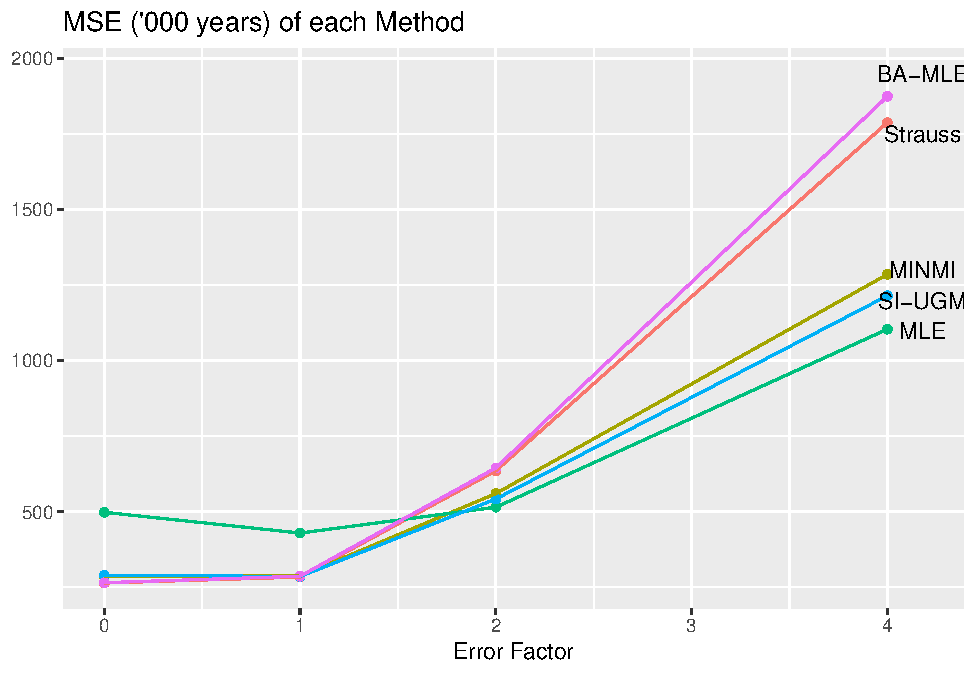
\includegraphics{sim_exp-results_files/figure-latex/unnamed-chunk-5-1.pdf}

\hypertarget{confidence-intervals}{%
\subsubsection{Confidence Intervals}\label{confidence-intervals}}

\begin{Shaded}
\begin{Highlighting}[]
\FunctionTok{options}\NormalTok{(}\AttributeTok{scipen=}\DecValTok{9}\NormalTok{)}
\ControlFlowTok{for}\NormalTok{ (metric }\ControlFlowTok{in} \FunctionTok{c}\NormalTok{(}\StringTok{"coverage"}\NormalTok{, }\StringTok{"avg\_width"}\NormalTok{, }\StringTok{"avg\_runtime"}\NormalTok{)) \{}
  \FunctionTok{print}\NormalTok{(}\FunctionTok{kable}\NormalTok{(}
\NormalTok{    performance.conf\_int\_estimates }\SpecialCharTok{\%\textgreater{}\%}
      \FunctionTok{select}\NormalTok{(}\FunctionTok{c}\NormalTok{(method, error\_factor, }\FunctionTok{one\_of}\NormalTok{(metric))) }\SpecialCharTok{\%\textgreater{}\%}
      \FunctionTok{pivot\_wider}\NormalTok{(}\AttributeTok{id\_cols =}\NormalTok{ method,}
                \AttributeTok{names\_from=}\NormalTok{error\_factor,}
                \AttributeTok{values\_from=}\FunctionTok{one\_of}\NormalTok{(metric),}
                \AttributeTok{names\_prefix=}\FunctionTok{paste}\NormalTok{(metric, }\StringTok{"| error = sigma*"}\NormalTok{)) }\SpecialCharTok{\%\textgreater{}\%}
      \FunctionTok{arrange}\NormalTok{(}\SpecialCharTok{!!}\FunctionTok{sym}\NormalTok{(}\FunctionTok{paste}\NormalTok{(metric, }\StringTok{"| error = sigma*0"}\NormalTok{)))}
\NormalTok{  ))}
\NormalTok{\}}
\end{Highlighting}
\end{Shaded}

\begin{tabular}{l|r|r|r|r}
\hline
method & coverage | error = sigma*0 & coverage | error = sigma*1 & coverage | error = sigma*2 & coverage | error = sigma*4\\
\hline
GRIWM & 0.000 & 0.156 & 0.212 & 0.260\\
\hline
GRIWM-corrected & 0.000 & 0.096 & 0.120 & 0.196\\
\hline
MINMI & 0.936 & 0.956 & 0.940 & 0.948\\
\hline
SI-UGM & 0.952 & 0.956 & 0.940 & 0.956\\
\hline
GB-RM & 0.956 & 0.948 & 0.948 & 0.952\\
\hline
\end{tabular}

\begin{tabular}{l|r|r|r|r}
\hline
method & avg\_width | error = sigma*0 & avg\_width | error = sigma*1 & avg\_width | error = sigma*2 & avg\_width | error = sigma*4\\
\hline
GRIWM & 0.000 & 1161.740 & 2191.180 & 4070.620\\
\hline
GRIWM-corrected & 0.000 & 1190.240 & 2242.436 & 4162.476\\
\hline
MINMI & 1910.220 & 2331.017 & 2948.932 & 4315.484\\
\hline
SI-UGM & 1949.626 & 2350.378 & 2972.823 & 4409.469\\
\hline
GB-RM & 2040.898 & 2361.442 & 3003.598 & 4420.989\\
\hline
\end{tabular}

\begin{tabular}{l|r|r|r|r}
\hline
method & avg\_runtime | error = sigma*0 & avg\_runtime | error = sigma*1 & avg\_runtime | error = sigma*2 & avg\_runtime | error = sigma*4\\
\hline
MINMI & 0.0000671 & 0.0014753 & 0.0018413 & 0.0012475\\
\hline
GB-RM & 0.0202166 & 0.0235130 & 0.0230765 & 0.0203415\\
\hline
GRIWM & 2.2955959 & 2.3225908 & 2.3258716 & 2.3208188\\
\hline
SI-UGM & 4.4242394 & 2.0293313 & 1.7308850 & 1.3886812\\
\hline
GRIWM-corrected & 14.2799933 & 14.3278799 & 14.2027869 & 14.2912016\\
\hline
\end{tabular}

\begin{Shaded}
\begin{Highlighting}[]
\NormalTok{performance.conf\_int\_estimates }\SpecialCharTok{\%\textgreater{}\%}
  
  \FunctionTok{ggplot}\NormalTok{(}\FunctionTok{aes}\NormalTok{(}\AttributeTok{x=}\FunctionTok{reorder}\NormalTok{(method, coverage, }\AttributeTok{descending=}\ConstantTok{TRUE}\NormalTok{), }\AttributeTok{y=}\NormalTok{coverage)) }\SpecialCharTok{+}
  \FunctionTok{geom\_col}\NormalTok{() }\SpecialCharTok{+}
  \FunctionTok{geom\_text}\NormalTok{(}\FunctionTok{aes}\NormalTok{(}\AttributeTok{label=}\NormalTok{scales}\SpecialCharTok{::}\FunctionTok{percent}\NormalTok{(coverage)), }\AttributeTok{position =} \FunctionTok{position\_dodge}\NormalTok{(.}\DecValTok{9}\NormalTok{), }\AttributeTok{vjust =} \FloatTok{1.5}\NormalTok{, }\AttributeTok{colour=}\StringTok{"white"}\NormalTok{) }\SpecialCharTok{+}
  \FunctionTok{labs}\NormalTok{(}\AttributeTok{x=}\ConstantTok{NULL}\NormalTok{, }\AttributeTok{y=}\StringTok{"\%"}\NormalTok{, }\AttributeTok{title=}\StringTok{"Coverage Probabilities"}\NormalTok{) }\SpecialCharTok{+}
  \FunctionTok{facet\_wrap}\NormalTok{(error\_factor }\SpecialCharTok{\textasciitilde{}}\NormalTok{.) }\SpecialCharTok{+}
  \FunctionTok{scale\_y\_continuous}\NormalTok{(}\AttributeTok{labels =}\NormalTok{ scales}\SpecialCharTok{::}\NormalTok{percent)}
\end{Highlighting}
\end{Shaded}

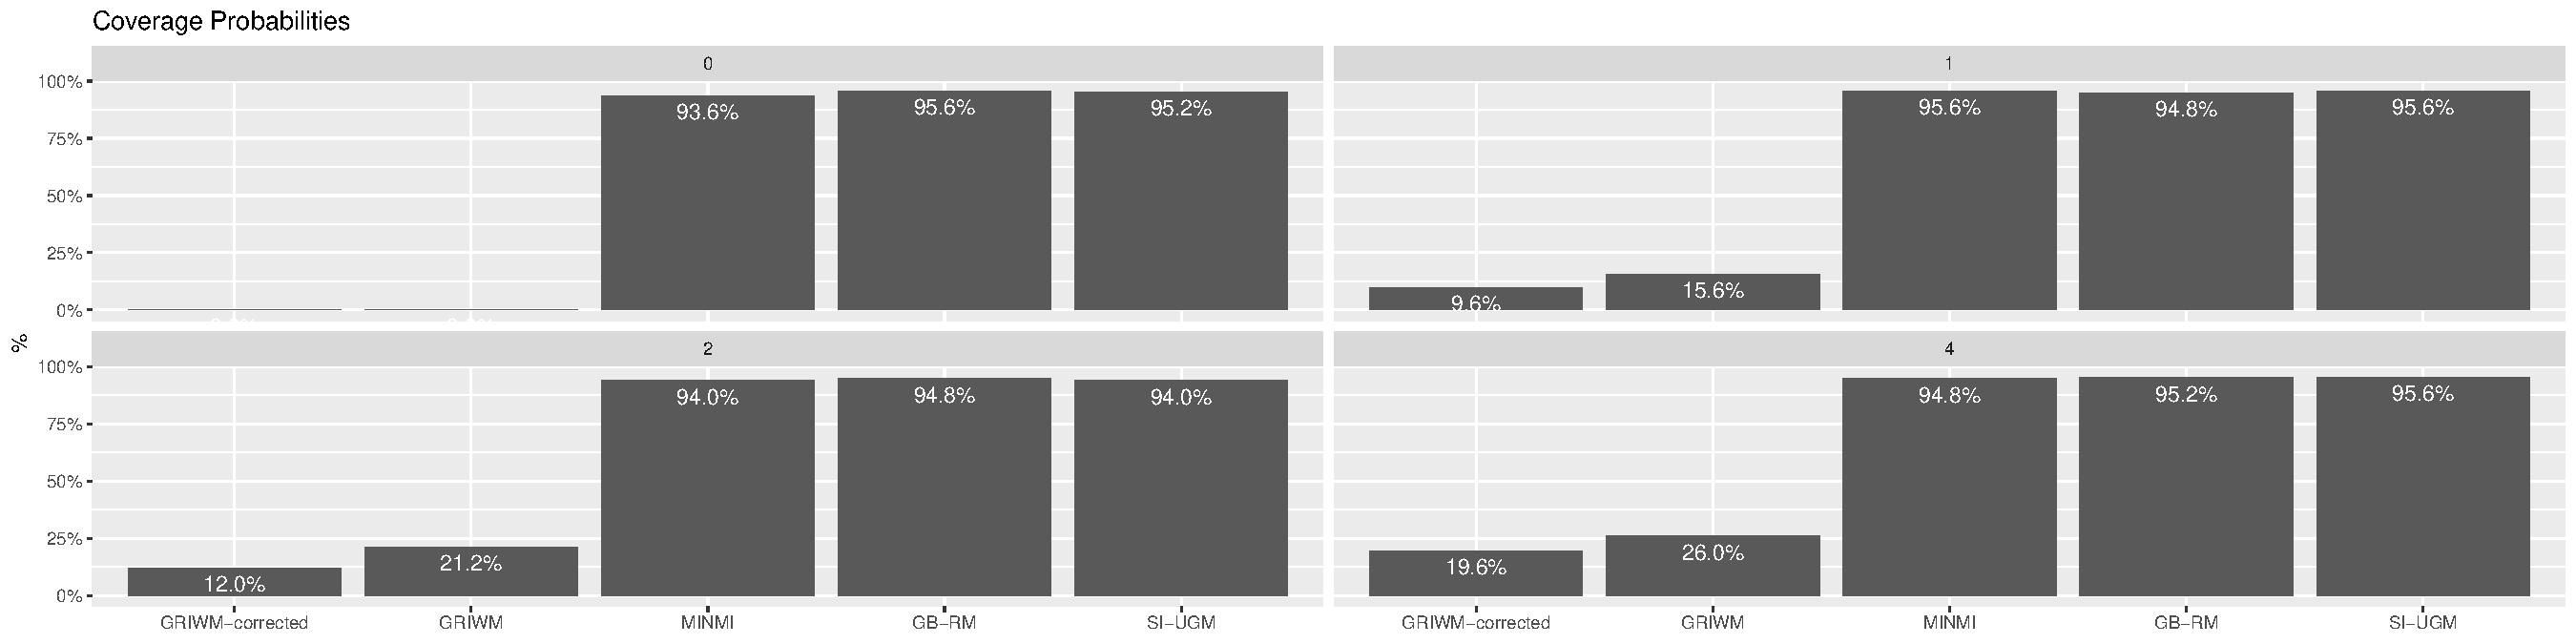
\includegraphics{sim_exp-results_files/figure-latex/unnamed-chunk-7-1.pdf}

\begin{Shaded}
\begin{Highlighting}[]
\NormalTok{estimates }\SpecialCharTok{\%\textgreater{}\%}
  \FunctionTok{filter}\NormalTok{(}\SpecialCharTok{!}\FunctionTok{is.na}\NormalTok{(lower)) }\SpecialCharTok{\%\textgreater{}\%}
  \FunctionTok{select}\NormalTok{(method, lower, point, upper) }\SpecialCharTok{\%\textgreater{}\%}
  \FunctionTok{pivot\_longer}\NormalTok{(}\AttributeTok{cols=}\FunctionTok{c}\NormalTok{(lower, point, upper)) }\SpecialCharTok{\%\textgreater{}\%}
  \FunctionTok{filter}\NormalTok{(}\SpecialCharTok{!}\FunctionTok{is.na}\NormalTok{(value)) }\SpecialCharTok{\%\textgreater{}\%}
  \FunctionTok{ggplot}\NormalTok{(}\FunctionTok{aes}\NormalTok{(}\AttributeTok{x=}\NormalTok{value, }\AttributeTok{fill=}\NormalTok{name)) }\SpecialCharTok{+}
  \FunctionTok{geom\_density}\NormalTok{(}\AttributeTok{alpha=}\FloatTok{0.25}\NormalTok{) }\SpecialCharTok{+}
  \FunctionTok{geom\_vline}\NormalTok{(}\FunctionTok{aes}\NormalTok{(}\AttributeTok{xintercept=}\NormalTok{theta.true)) }\SpecialCharTok{+}
  \FunctionTok{facet\_wrap}\NormalTok{(method }\SpecialCharTok{\textasciitilde{}}\NormalTok{ .)}
\end{Highlighting}
\end{Shaded}

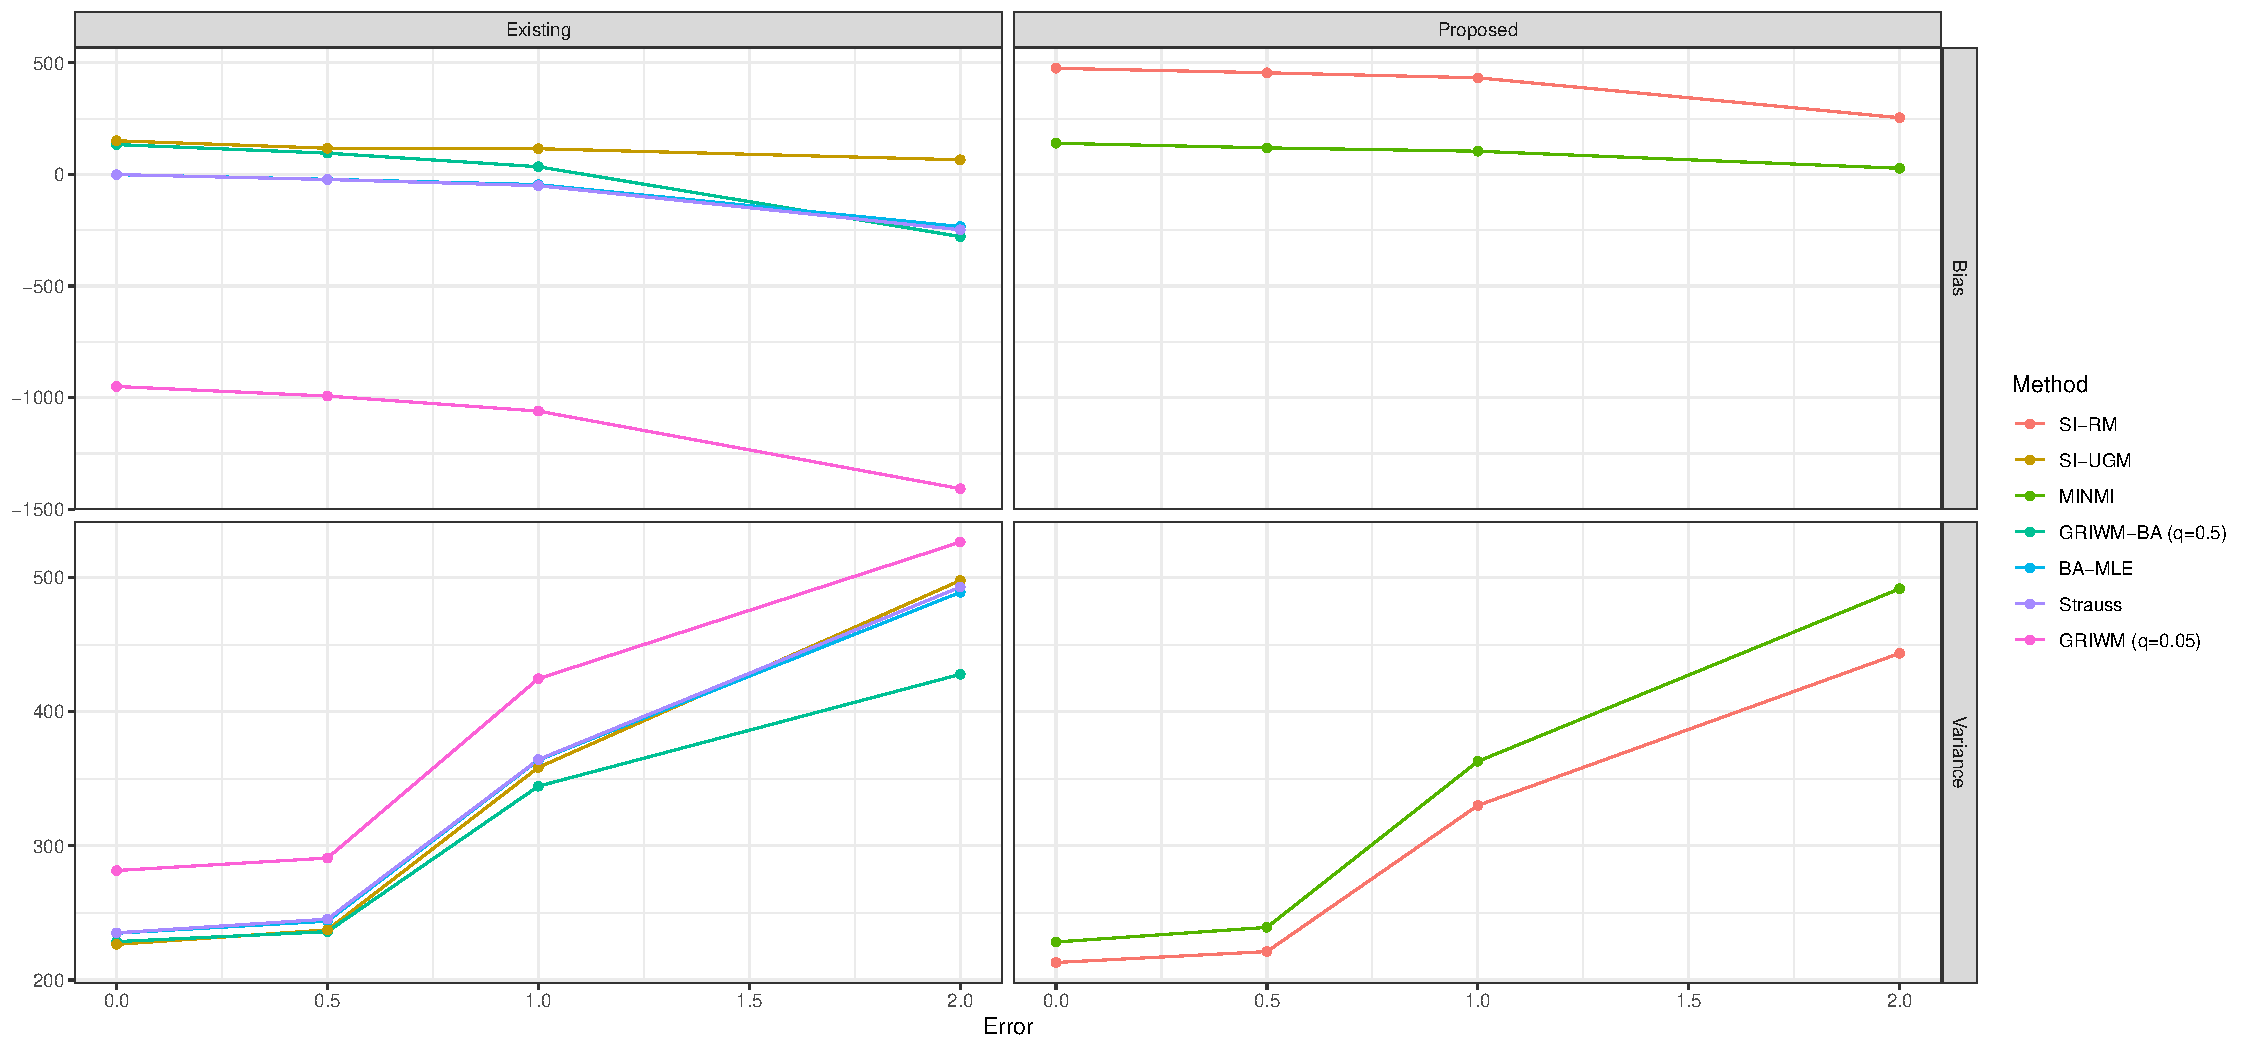
\includegraphics{sim_exp-results_files/figure-latex/unnamed-chunk-8-1.pdf}

\end{document}
